\documentclass{beamer}\usepackage[]{graphicx}\usepackage[]{color}
% maxwidth is the original width if it is less than linewidth
% otherwise use linewidth (to make sure the graphics do not exceed the margin)
\makeatletter
\def\maxwidth{ %
  \ifdim\Gin@nat@width>\linewidth
    \linewidth
  \else
    \Gin@nat@width
  \fi
}
\makeatother

\definecolor{fgcolor}{rgb}{0.345, 0.345, 0.345}
\newcommand{\hlnum}[1]{\textcolor[rgb]{0.686,0.059,0.569}{#1}}%
\newcommand{\hlstr}[1]{\textcolor[rgb]{0.192,0.494,0.8}{#1}}%
\newcommand{\hlcom}[1]{\textcolor[rgb]{0.678,0.584,0.686}{\textit{#1}}}%
\newcommand{\hlopt}[1]{\textcolor[rgb]{0,0,0}{#1}}%
\newcommand{\hlstd}[1]{\textcolor[rgb]{0.345,0.345,0.345}{#1}}%
\newcommand{\hlkwa}[1]{\textcolor[rgb]{0.161,0.373,0.58}{\textbf{#1}}}%
\newcommand{\hlkwb}[1]{\textcolor[rgb]{0.69,0.353,0.396}{#1}}%
\newcommand{\hlkwc}[1]{\textcolor[rgb]{0.333,0.667,0.333}{#1}}%
\newcommand{\hlkwd}[1]{\textcolor[rgb]{0.737,0.353,0.396}{\textbf{#1}}}%
\let\hlipl\hlkwb

\usepackage{framed}
\makeatletter
\newenvironment{kframe}{%
 \def\at@end@of@kframe{}%
 \ifinner\ifhmode%
  \def\at@end@of@kframe{\end{minipage}}%
  \begin{minipage}{\columnwidth}%
 \fi\fi%
 \def\FrameCommand##1{\hskip\@totalleftmargin \hskip-\fboxsep
 \colorbox{shadecolor}{##1}\hskip-\fboxsep
     % There is no \\@totalrightmargin, so:
     \hskip-\linewidth \hskip-\@totalleftmargin \hskip\columnwidth}%
 \MakeFramed {\advance\hsize-\width
   \@totalleftmargin\z@ \linewidth\hsize
   \@setminipage}}%
 {\par\unskip\endMakeFramed%
 \at@end@of@kframe}
\makeatother

\definecolor{shadecolor}{rgb}{.97, .97, .97}
\definecolor{messagecolor}{rgb}{0, 0, 0}
\definecolor{warningcolor}{rgb}{1, 0, 1}
\definecolor{errorcolor}{rgb}{1, 0, 0}
\newenvironment{knitrout}{}{} % an empty environment to be redefined in TeX

\usepackage{alltt}
\usetheme{Boadilla}

\makeatother
\setbeamertemplate{footline}
{
    \leavevmode%
    \hbox{%
    \begin{beamercolorbox}[wd=.4\paperwidth,ht=2.25ex,dp=1ex,center]{author in head/foot}%
        \usebeamerfont{author in head/foot}\insertshortauthor
    \end{beamercolorbox}%
    \begin{beamercolorbox}[wd=.55\paperwidth,ht=2.25ex,dp=1ex,center]{title in head/foot}%
        \usebeamerfont{title in head/foot}\insertshorttitle
    \end{beamercolorbox}%
    \begin{beamercolorbox}[wd=.05\paperwidth,ht=2.25ex,dp=1ex,center]{date in head/foot}%
        \insertframenumber{}
    \end{beamercolorbox}}%
    \vskip0pt%
}
\makeatletter
\setbeamertemplate{navigation symbols}{}

\usepackage[T1]{fontenc}
\usepackage{lmodern}
\usepackage{amssymb,amsmath,bm}
\renewcommand{\familydefault}{\sfdefault}

\DeclareMathOperator*{\Cov}{Cov}

\usepackage{mathtools}
\usepackage{graphicx}
\usepackage{threeparttable}
\usepackage{booktabs}
\usepackage{siunitx}
\sisetup{parse-numbers=false}

\setlength{\OuterFrameSep}{-2pt}
\makeatletter
\preto{\@verbatim}{\topsep=-10pt \partopsep=-10pt }
\makeatother

\title[Week 2:\ R Tutorial]{Week 2:\ R Tutorial}
\author[ResEcon 703:\ Advanced Econometrics]{ResEcon 703:\ Topics in Advanced Econometrics}
\date{Matt Woerman\\University of Massachusetts Amherst}
\IfFileExists{upquote.sty}{\usepackage{upquote}}{}
\begin{document}


{\setbeamertemplate{footline}{} 
\begin{frame}[noframenumbering]
    \titlepage
\end{frame}
}

\begin{frame}\frametitle{Agenda}
    Last week
    \begin{itemize}
        \item Structural estimation
    \end{itemize}
    \vspace{2ex}
    This week's topics
    \begin{itemize}
    	\item \hyperlink{page.\getpagerefnumber{resources}}{R resources}
        \item \hyperlink{page.\getpagerefnumber{objects}}{Objects in R}
        \item \hyperlink{page.\getpagerefnumber{functions}}{Functions and packages in R}
        \item \hyperlink{page.\getpagerefnumber{math}}{Math and statistics in R}
        \item \hyperlink{page.\getpagerefnumber{data}}{Data in R}
        \item \hyperlink{page.\getpagerefnumber{examples}}{R examples}
    \end{itemize}
    \vspace{2ex}
    This week's ``reading''
    \begin{itemize}
        \item R \texttt{swirl} interactive tutorials
    \end{itemize}
\end{frame}

\section{R Resources}
\label{resources}
\begin{frame}\frametitle{}
    \vfill
    \centering
    \begin{beamercolorbox}[center]{title}
        \Large R Resources
    \end{beamercolorbox}
    \vfill
\end{frame}

\begin{frame}\frametitle{Hat Tips}
    This lecture is inspired heavily by notes and slides created by
    \begin{itemize}
        \item \href{https://www.fionaburlig.com/}{Fiona Burlig, University of Chicago}
        \item \href{https://grantmcdermott.com/}{Grant McDermott, University of Oregon}
        \item \href{http://edrub.in/}{Ed Rubin, University of Oregon}
    \end{itemize}
    \vspace{3ex}
    Many thanks to them for generously making their course materials available online for all!
\end{frame}

\begin{frame}\frametitle{Installing R}
    Installing R is \emph{usually} straightforward \\
    \vspace{1ex}
    \begin{tabular}{@{\extracolsep{-2ex}} c l}
        \begin{tabular}{c}
            
\includegraphics[width=0.05\linewidth]{r}
        \end{tabular} & 
        \begin{tabular}{l}
            \parbox{0.9\linewidth}{
            \href{https://cran.r-project.org/}{Download (\texttt{cran.r-project.org})} and install R
            }
        \end{tabular}
    \end{tabular} \\
    \vspace{1ex}
    \begin{tabular}{@{\extracolsep{-2ex}} c l}
        \begin{tabular}{c}
            
\includegraphics[width=0.05\linewidth]{rstudio}
        \end{tabular} & 
        \begin{tabular}{l}
            \parbox{0.9\linewidth}{
            \href{https://www.rstudio.com/products/rstudio/download/}{Download (\texttt{www.rstudio.com/products/rstudio/download})}\\ and install RStudio Desktop (Open Source License)
            }
        \end{tabular}
    \end{tabular} \\
    \vspace{3ex}
    What is the difference between R and RStudio? \\
    \vspace{1ex}
    \begin{tabular}{@{\extracolsep{-2ex}} c l}
        \begin{tabular}{c}
            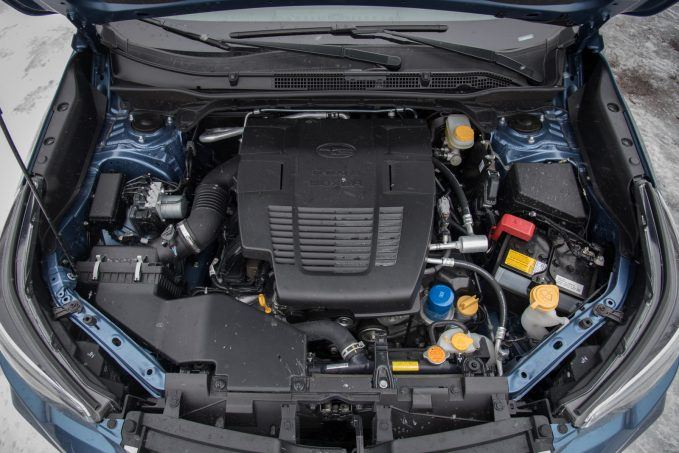
\includegraphics[width=0.25\linewidth]{engine}
        \end{tabular} & 
        \begin{tabular}{l}
            \parbox{0.65\linewidth}{
            R is like a car's engine. It is the program that powers your data analysis.
            }
        \end{tabular}
    \end{tabular} \\
    \vspace{1ex}
    \begin{tabular}{@{\extracolsep{-2ex}} c l}
        \begin{tabular}{c}
            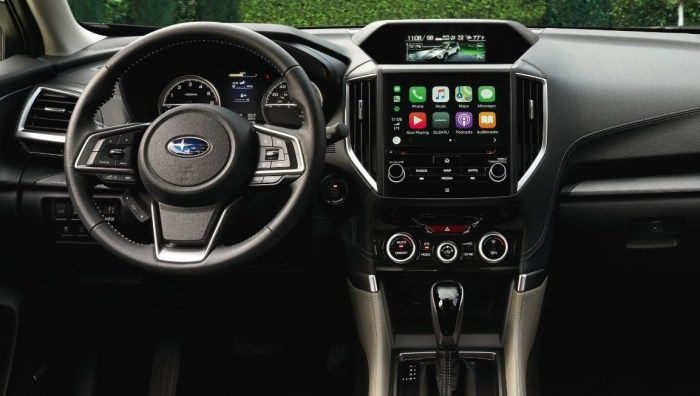
\includegraphics[width=0.25\linewidth]{dashboard}
        \end{tabular} & 
        \begin{tabular}{l}
            \parbox{0.65\linewidth}{
            RStudio is like a car's dashboard. It is the program you interact with to harness the power of your ``engine.''
            }
        \end{tabular}
    \end{tabular}
\end{frame}

\begin{frame}[fragile]\frametitle{R \texttt{swirl} Interactive Tutorials}
    \texttt{swirl} is an R package that interactively teaches you how to use R
    \begin{itemize}
    	\item Information available here: \href{https://swirlstats.com/}{\texttt{swirlstats.com}}
    \end{itemize}
    \vspace{2ex}
\begin{knitrout}\footnotesize
\definecolor{shadecolor}{rgb}{0.969, 0.969, 0.969}\color{fgcolor}\begin{kframe}
\begin{alltt}
\hlcom{## Install swirl package}
\hlkwd{install.packages}\hlstd{(}\hlstr{'swirl'}\hlstd{)}
\hlcom{## Load swirl package}
\hlkwd{library}\hlstd{(swirl)}
\hlcom{## Install swirl tutorials}
\hlkwd{install_course}\hlstd{(}\hlstr{'R Programming'}\hlstd{)}
\hlkwd{install_course}\hlstd{(}\hlstr{'Getting and Cleaning Data'}\hlstd{)}
\hlkwd{install_course}\hlstd{(}\hlstr{'Advanced R Programming'}\hlstd{)}
\hlcom{## Start swirl tutorials}
\hlkwd{swirl}\hlstd{()}
\end{alltt}
\end{kframe}
\end{knitrout}
    \vspace{2ex}
    These three \texttt{swirl} tutorials (R Programming, Getting and Cleaning Data, and Advanced R Programming) introduce the main R concepts we will use in this course
\end{frame}

\begin{frame}\frametitle{More R Resources}
    These links provide a variety of perspectives and topics related to using R for statistical analysis, all of which may be useful as you learn to use R for structural estimation in this course
    \begin{itemize}
        \item \href{https://www.datacamp.com/courses/free-introduction-to-r}{DataCamp's Introduction to R}
        \item \href{https://r4ds.had.co.nz/}{R for Data Science book}
        \item \href{https://adv-r.hadley.nz/}{Advanced R book}
        \item \href{https://github.com/edrubin/EC525S19}{Ed Rubin's Econometrics lab slides}
        \item \href{http://edrub.in/ARE212/notes.html}{Ed Rubin's Econometrics section notes}
        \item \href{https://www.fionaburlig.com/teaching/are212}{Fiona Burlig's Econometrics section notes} (warning: puns ahead)
        \item \href{https://github.com/uo-ec607/lectures}{Grant McDermott's Data Science for Economists lecture slides}
    \end{itemize}
\end{frame}

\begin{frame}\frametitle{Some Complements to R}
    \LaTeX\ and \texttt{knitr}
    \begin{itemize}
        \item \href{https://www.latex-project.org/}{\LaTeX\ (\texttt{www.latex-project.org})}: Typesetting system with great functionality for technical and scientific documents
        \item \href{https://yihui.name/knitr/}{\texttt{knitr} (\texttt{yihui.name/knitr})}: R package that integrates R code and output into \LaTeX\ documents (or HTML, Markdown, etc.)
    \end{itemize}
    \vspace{3ex}
    Git, GitHub, and SmartGit
    \begin{itemize}
        \item \href{https://git-scm.com/}{Git (\texttt{git-scm.com})}: Version control system
        \item \href{https://github.com/}{GitHub (\texttt{github.com})}: Hosting platform for Git
        \begin{itemize}
            \item Some alternatives exist: BitBucket, SourceForge, GitLab
        \end{itemize}
        \item \href{https://www.syntevo.com/smartgit/}{SmartGit (\texttt{www.syntevo.com/smartgit})}: GUI client for Git
        \begin{itemize}
            \item Many alternatives exist: GitHub Desktop, GitKraken, SourceTree
        \end{itemize}
    \end{itemize}
\end{frame}

\section{Objects in R}
\label{objects}
\begin{frame}\frametitle{}
    \vfill
    \centering
    \begin{beamercolorbox}[center]{title}
        \Large Objects in R
    \end{beamercolorbox}
    \vfill
\end{frame}

\begin{frame}[fragile]\frametitle{Object Basics}
    Everything is an object, and every object has a name and value
\begin{knitrout}\footnotesize
\definecolor{shadecolor}{rgb}{0.969, 0.969, 0.969}\color{fgcolor}\begin{kframe}
\begin{alltt}
\hlcom{## Assign a value of 1 to an object called a}
\hlstd{a} \hlkwb{<-} \hlnum{1}
\hlcom{## Assign a value of 2 to an object called b}
\hlstd{b} \hlkwb{<-} \hlnum{2}
\hlcom{## You use these objects in operations and functions}
\hlstd{a} \hlopt{+} \hlstd{b}
\end{alltt}
\begin{verbatim}
## [1] 3
\end{verbatim}
\begin{alltt}
\hlcom{## Assign object c to have a value equal to a + b}
\hlstd{c} \hlkwb{<-} \hlstd{a} \hlopt{+} \hlstd{b}
\hlstd{c}
\end{alltt}
\begin{verbatim}
## [1] 3
\end{verbatim}
\end{kframe}
\end{knitrout}
\end{frame}

\begin{frame}\frametitle{Classes, Types, and Structures}
    Every object has a type
    \begin{itemize}
        \item Numeric: \texttt{1}, \texttt{0.5}, \texttt{2/3}, \texttt{pi}
        \item Character: \texttt{"Hello"}, \texttt{"cruel world"}, \texttt{"Metrics is fun!"}
        \item Logical: \texttt{TRUE}, \texttt{FALSE}, \texttt{T}, \texttt{F}
    \end{itemize}
    \vspace{2ex}
    Every object has a structure
    \begin{itemize}
        \item Vector
        \item Matrix
        \item List
        \item Data frame
    \end{itemize}
    \vspace{2ex}
    \texttt{class()}, \texttt{typeof()}, \texttt{str()} give information about an object
\end{frame}

\begin{frame}[fragile]\frametitle{Vectors}
    A vector is a collection of elements of the same type
    \begin{itemize}
        \item \texttt{c()} combines elements into a vector
        \item \texttt{seq()} and \texttt{:} create sequential vectors of numeric elements
    \end{itemize}
\begin{knitrout}\footnotesize
\definecolor{shadecolor}{rgb}{0.969, 0.969, 0.969}\color{fgcolor}\begin{kframe}
\begin{alltt}
\hlcom{## Create a numeric vector}
\hlkwd{c}\hlstd{(}\hlnum{1}\hlstd{,} \hlnum{1}\hlstd{,} \hlnum{2}\hlstd{,} \hlnum{3}\hlstd{,} \hlnum{5}\hlstd{,} \hlnum{8}\hlstd{,} \hlnum{13}\hlstd{)}
\end{alltt}
\begin{verbatim}
## [1]  1  1  2  3  5  8 13
\end{verbatim}
\begin{alltt}
\hlcom{## Create a sequential vector}
\hlnum{0}\hlopt{:}\hlnum{9}
\end{alltt}
\begin{verbatim}
##  [1] 0 1 2 3 4 5 6 7 8 9
\end{verbatim}
\begin{alltt}
\hlcom{## Create a character vector}
\hlkwd{c}\hlstd{(}\hlstr{'Hello'}\hlstd{,} \hlstr{'world'}\hlstd{)}
\end{alltt}
\begin{verbatim}
## [1] "Hello" "world"
\end{verbatim}
\end{kframe}
\end{knitrout}
    \vspace{2ex} 
    If you combine elements of different types, R will convert some
\begin{knitrout}\footnotesize
\definecolor{shadecolor}{rgb}{0.969, 0.969, 0.969}\color{fgcolor}\begin{kframe}
\begin{alltt}
\hlcom{## Create a vector with numeric, character, and logical elements}
\hlkwd{c}\hlstd{(}\hlnum{1}\hlstd{,} \hlstr{'Hello'}\hlstd{,} \hlnum{3}\hlstd{,} \hlstr{'world'}\hlstd{,} \hlnum{TRUE}\hlstd{)}
\end{alltt}
\begin{verbatim}
## [1] "1"     "Hello" "3"     "world" "TRUE"
\end{verbatim}
\end{kframe}
\end{knitrout}
\end{frame}

\begin{frame}[fragile]\frametitle{Matrices}
    A matrix is a collection of elements of the same type arranged in two dimensions \\
    \vspace{3ex}
    \texttt{matrix()} arranges a vector of data into a matrix
    \begin{itemize}
        \item \texttt{data}: Vector of data to create matrix
        \item \texttt{nrow} or \texttt{ncol}: Number of rows or columns in the matrix
        \item \texttt{byrow}: Logical indicating how to arrange data
    \end{itemize}
\begin{knitrout}\footnotesize
\definecolor{shadecolor}{rgb}{0.969, 0.969, 0.969}\color{fgcolor}\begin{kframe}
\begin{alltt}
\hlcom{## Create a 2 (rows) x 5 (columns) matrix of 1:10 arranged by row}
\hlkwd{matrix}\hlstd{(}\hlkwc{data} \hlstd{=} \hlnum{1}\hlopt{:}\hlnum{10}\hlstd{,} \hlkwc{nrow} \hlstd{=} \hlnum{2}\hlstd{,} \hlkwc{byrow} \hlstd{=} \hlnum{TRUE}\hlstd{)}
\end{alltt}
\begin{verbatim}
##      [,1] [,2] [,3] [,4] [,5]
## [1,]    1    2    3    4    5
## [2,]    6    7    8    9   10
\end{verbatim}
\end{kframe}
\end{knitrout}
\end{frame}

\begin{frame}[fragile]\frametitle{Lists}
    A list is a collection of elements that can have different types and different structures \\
    \vspace{3ex}
    \texttt{list()} combines elements into a list
\begin{knitrout}\footnotesize
\definecolor{shadecolor}{rgb}{0.969, 0.969, 0.969}\color{fgcolor}\begin{kframe}
\begin{alltt}
\hlcom{## Create a list with a numeric vector, matrix, and character vector}
\hlkwd{list}\hlstd{(}\hlkwd{c}\hlstd{(}\hlnum{2}\hlstd{,} \hlnum{4}\hlstd{,} \hlnum{6}\hlstd{,} \hlnum{8}\hlstd{),} \hlkwd{matrix}\hlstd{(}\hlnum{1}\hlopt{:}\hlnum{4}\hlstd{,} \hlnum{2}\hlstd{),} \hlkwd{c}\hlstd{(}\hlstr{'a'}\hlstd{,} \hlstr{'b'}\hlstd{,} \hlstr{'c'}\hlstd{))}
\end{alltt}
\begin{verbatim}
## [[1]]
## [1] 2 4 6 8
## 
## [[2]]
##      [,1] [,2]
## [1,]    1    3
## [2,]    2    4
## 
## [[3]]
## [1] "a" "b" "c"
\end{verbatim}
\end{kframe}
\end{knitrout}
\end{frame}

\begin{frame}[fragile]\frametitle{Data Frames}
    A data frame is a structured table of data arranged in two dimensions
    \begin{itemize}
        \item Each column is a ``variable'' and each row is an ``observation''
        \item Technically, a data frame is a list of named vectors of the same length
        \begin{itemize}
            \item Each vector is a ``variable''
            \item The length of each vector equals the number of ``observations''
        \end{itemize}
    \end{itemize}
    \vspace{3ex}
    \texttt{data.frame()} combines vectors into a data frame
\begin{knitrout}\footnotesize
\definecolor{shadecolor}{rgb}{0.969, 0.969, 0.969}\color{fgcolor}\begin{kframe}
\begin{alltt}
\hlcom{## Create a date frame with 4 variables and 3 observations}
\hlkwd{data.frame}\hlstd{(}\hlkwc{x} \hlstd{=} \hlnum{0}\hlopt{:}\hlnum{2}\hlstd{,} \hlkwc{y} \hlstd{=} \hlkwd{c}\hlstd{(}\hlnum{2}\hlstd{,} \hlnum{4}\hlstd{,} \hlnum{8}\hlstd{),} \hlkwc{z} \hlstd{=} \hlkwd{c}\hlstd{(}\hlnum{1}\hlstd{,} \hlnum{5}\hlstd{,} \hlnum{7}\hlstd{),} \hlkwc{w} \hlstd{=} \hlkwd{c}\hlstd{(}\hlstr{'a'}\hlstd{,} \hlstr{'b'}\hlstd{,} \hlstr{'c'}\hlstd{))}
\end{alltt}
\begin{verbatim}
##   x y z w
## 1 0 2 1 a
## 2 1 4 5 b
## 3 2 8 7 c
\end{verbatim}
\end{kframe}
\end{knitrout}
\end{frame}

\section{Functions and Packages in R}
\label{functions}
\begin{frame}\frametitle{}
    \vfill
    \centering
    \begin{beamercolorbox}[center]{title}
        \Large Functions and Packages in R
    \end{beamercolorbox}
    \vfill
\end{frame}

\begin{frame}\frametitle{Functions}
    A function in R
    \begin{enumerate}
        \item Takes some inputs
        \item Performs some internal tasks
        \item Returns some output
    \end{enumerate}
    \vspace{2ex}
    We have already seen some examples of functions
    \begin{itemize}
        \item \texttt{matrix()}
        \begin{enumerate}
            \item Takes a vector of data, information about the size of the matrix, and information about the arrangement of the matrix
            \item Arranges the data in the way specified by the other inputs
            \item Returns a matrix object
        \end{enumerate}
    \end{itemize}
    \vspace{2ex}
    Use \texttt{?} (e.g., \texttt{?matrix}) to get the help file for a function
\end{frame}

\begin{frame}[fragile]\frametitle{Function Inputs}
    Many functions have default inputs so you do not have to specify all the arguments
    \begin{itemize}
        \item These defaults are shown when you look at the function help file
    \end{itemize}
    \vspace{2ex}
    Use \texttt{?matrix} to see the set of default inputs for the \texttt{matrix()} function
\begin{knitrout}\footnotesize
\definecolor{shadecolor}{rgb}{0.969, 0.969, 0.969}\color{fgcolor}\begin{kframe}
\begin{alltt}
\hlcom{## Matrix function default inputs}
\hlkwd{matrix}\hlstd{(}\hlkwc{data} \hlstd{=} \hlnum{NA}\hlstd{,} \hlkwc{nrow} \hlstd{=} \hlnum{1}\hlstd{,} \hlkwc{ncol} \hlstd{=} \hlnum{1}\hlstd{,} \hlkwc{byrow} \hlstd{=} \hlnum{FALSE}\hlstd{,} \hlkwc{dimnames} \hlstd{=} \hlkwa{NULL}\hlstd{)}
\end{alltt}
\end{kframe}
\end{knitrout}
    \vspace{2ex}
    So the default inputs would create a 1 $\times$ 1 matrix of \texttt{NA}
\begin{knitrout}\footnotesize
\definecolor{shadecolor}{rgb}{0.969, 0.969, 0.969}\color{fgcolor}\begin{kframe}
\begin{alltt}
\hlcom{## Create matrix with default inputs}
\hlkwd{matrix}\hlstd{()}
\end{alltt}
\begin{verbatim}
##      [,1]
## [1,]   NA
\end{verbatim}
\end{kframe}
\end{knitrout}
    \vspace{2ex}
    Inputs can also be highly flexible
    \begin{itemize}
        \item \texttt{c()} allows for any number of arguments (as long as you have the memory to create a vector of the specified length)
    \end{itemize}
\end{frame}

\begin{frame}\frametitle{User-Defined Functions}
    R makes it easy to define your own functions \\
    \vspace{2ex}
    Why create your own functions?
    \begin{itemize}
        \item You are performing the same task more than once
        \item You want to make it easier to parallelize your code
        \item You want to make your code more readable
    \end{itemize}
    \vspace{2ex}
    How to create your own functions using \texttt{function()\char '173 \char '175}
    \begin{enumerate}
        \item Specify the inputs in the \texttt{()}
        \item Write the code for the function tasks in the \texttt{\char '173 \char '175}
        \item Specify the output using \texttt{return()} in the \texttt{\char '173 \char '175}
    \end{enumerate}
\end{frame}

\begin{frame}[fragile]\frametitle{Function Example}
    Make a function that calculates the mean sum of squares of three numbers \\
\begin{knitrout}\footnotesize
\definecolor{shadecolor}{rgb}{0.969, 0.969, 0.969}\color{fgcolor}\begin{kframe}
\begin{alltt}
\hlcom{## Define a function that calculates the MSS from three inputs}
\hlstd{mean_sum_squares} \hlkwb{<-} \hlkwa{function}\hlstd{(}\hlkwc{num1}\hlstd{,} \hlkwc{num2}\hlstd{,} \hlkwc{num3}\hlstd{)\{}
  \hlcom{## Calculate the mean sum of squares}
  \hlstd{mss} \hlkwb{<-} \hlstd{(num1}\hlopt{^}\hlnum{2} \hlopt{+} \hlstd{num2}\hlopt{^}\hlnum{2} \hlopt{+} \hlstd{num3}\hlopt{^}\hlnum{2}\hlstd{)} \hlopt{/} \hlnum{3}
  \hlcom{## Return the answer}
  \hlkwd{return}\hlstd{(mss)}
\hlstd{\}}
\end{alltt}
\end{kframe}
\end{knitrout}
    \vspace{1ex}
    Try it out
\begin{knitrout}\footnotesize
\definecolor{shadecolor}{rgb}{0.969, 0.969, 0.969}\color{fgcolor}\begin{kframe}
\begin{alltt}
\hlcom{## Calculate the mean sum of squares of 1, 2, and 3}
\hlkwd{mean_sum_squares}\hlstd{(}\hlnum{1}\hlstd{,} \hlnum{2}\hlstd{,} \hlnum{3}\hlstd{)}
\end{alltt}
\begin{verbatim}
## [1] 4.666667
\end{verbatim}
\end{kframe}
\end{knitrout}
    \vspace{1ex}
    What if we want a default argument?
\begin{knitrout}\footnotesize
\definecolor{shadecolor}{rgb}{0.969, 0.969, 0.969}\color{fgcolor}\begin{kframe}
\begin{alltt}
\hlcom{## Make 3 the default input for the third argument}
mean_sum_squares <- \hlkwd{function}(num1, num2, num3 = 3)
\end{alltt}
\end{kframe}
\end{knitrout}
    \vspace{1ex}
    What if we want a flexible number of inputs?
    \begin{itemize}
        \item That is a little more complicated and context-specific\ldots
    \end{itemize}
\end{frame}

\begin{frame}\frametitle{Packages}
    A package is a bundle of code, documentation, and data that has been created and distributed by another R user
    \begin{itemize}
        \item More than 16,000 packages are available on CRAN, the official repository of R packages 
    \end{itemize}
    \vspace{2ex}
    What is so great about packages?
    \begin{itemize}
        \item Packages greatly increase the functionality available to you through ``canned'' routines
        \item Packages are open source
        \begin{itemize}
            \item A package can be created by anyone, even you!
            \item You can see the source code in any package
        \end{itemize}
        \item Some packages have vignettes that provide detailed examples for using the package's functionality
    \end{itemize}
    \vspace{2ex}
    Any problems to be aware of?
    \begin{itemize}
        \item A package can be created by anyone, so \emph{caveat utilitor} (user beware)
    \end{itemize}
\end{frame}

\begin{frame}[fragile]\frametitle{Using Packages}
    First download a package from CRAN using \texttt{install.packages()}
\begin{knitrout}\footnotesize
\definecolor{shadecolor}{rgb}{0.969, 0.969, 0.969}\color{fgcolor}\begin{kframe}
\begin{alltt}
\hlcom{## Install a few packages we will use in this course}
\hlkwd{install.packages}\hlstd{(}\hlkwd{c}\hlstd{(}\hlstr{'tidyverse'}\hlstd{,} \hlstr{'mlogit'}\hlstd{,} \hlstr{'gmm'}\hlstd{))}
\end{alltt}
\end{kframe}
\end{knitrout}
    \vspace{3ex}
    Then load the package into your R session using \texttt{library()}
\begin{knitrout}\footnotesize
\definecolor{shadecolor}{rgb}{0.969, 0.969, 0.969}\color{fgcolor}\begin{kframe}
\begin{alltt}
\hlcom{## Load those packages}
\hlkwd{library}\hlstd{(tidyverse)}
\hlkwd{library}\hlstd{(mlogit)}
\hlkwd{library}\hlstd{(gmm)}
\end{alltt}
\end{kframe}
\end{knitrout}
    \vspace{3ex}
    Update packages occasionally using \texttt{update.packages()}
\end{frame}

\begin{frame}\frametitle{Recommended Packages}
    Packages we will use in this course
    \begin{itemize}
        \item \texttt{tidyverse}
        \begin{itemize}
            \item Collection of packages that improve data analysis and visualization
        \end{itemize}
        \item \texttt{mlogit}
        \begin{itemize}
            \item Estimating multinomial logit models
        \end{itemize}
        \item \texttt{gmm}
        \begin{itemize}
            \item Generalized method of moments estimation
        \end{itemize}
    \end{itemize}
    \vspace{0.5ex}
    Other good packages
    \begin{itemize}
        \item \texttt{glue}
        \begin{itemize}
            \item Character functions
        \end{itemize}
        \item \texttt{lubridate}
        \begin{itemize}
            \item Date and time functions
        \end{itemize}
        \item \texttt{lfe}
        \begin{itemize}
            \item Fixed effects models
        \end{itemize}
        \item \texttt{furrr}
        \begin{itemize}
            \item Parallelization
        \end{itemize}
    \end{itemize}
\end{frame}

\section{Math and Statistics in R}
\label{math}
\begin{frame}\frametitle{}
    \vfill
    \centering
    \begin{beamercolorbox}[center]{title}
        \Large Math and Statistics in R
    \end{beamercolorbox}
    \vfill
\end{frame}

\begin{frame}[fragile]\frametitle{Math Operations}
\begin{knitrout}\footnotesize
\definecolor{shadecolor}{rgb}{0.969, 0.969, 0.969}\color{fgcolor}\begin{kframe}
\begin{alltt}
\hlcom{## Addition}
\hlstd{a} \hlopt{+} \hlstd{b}
\end{alltt}
\begin{verbatim}
## [1] 3
\end{verbatim}
\begin{alltt}
\hlcom{## Subtraction}
\hlstd{a} \hlopt{-} \hlstd{b}
\end{alltt}
\begin{verbatim}
## [1] -1
\end{verbatim}
\begin{alltt}
\hlcom{## Multiplication}
\hlstd{a} \hlopt{*} \hlstd{b}
\end{alltt}
\begin{verbatim}
## [1] 2
\end{verbatim}
\begin{alltt}
\hlcom{## Division}
\hlstd{a} \hlopt{/} \hlstd{b}
\end{alltt}
\begin{verbatim}
## [1] 0.5
\end{verbatim}
\begin{alltt}
\hlcom{## Exponents}
\hlstd{a}\hlopt{^}\hlstd{b}
\end{alltt}
\begin{verbatim}
## [1] 1
\end{verbatim}
\end{kframe}
\end{knitrout}
\end{frame}

\begin{frame}[fragile]\frametitle{Math Functions}
\begin{knitrout}\footnotesize
\definecolor{shadecolor}{rgb}{0.969, 0.969, 0.969}\color{fgcolor}\begin{kframe}
\begin{alltt}
\hlcom{## Absolute value}
\hlkwd{abs}\hlstd{(a} \hlopt{-} \hlstd{b)}
\end{alltt}
\begin{verbatim}
## [1] 1
\end{verbatim}
\begin{alltt}
\hlcom{## Exponential}
\hlkwd{exp}\hlstd{(a)}
\end{alltt}
\begin{verbatim}
## [1] 2.718282
\end{verbatim}
\begin{alltt}
\hlcom{## Square root}
\hlkwd{sqrt}\hlstd{(b)}
\end{alltt}
\begin{verbatim}
## [1] 1.414214
\end{verbatim}
\begin{alltt}
\hlcom{## Natural log}
\hlkwd{log}\hlstd{(b)}
\end{alltt}
\begin{verbatim}
## [1] 0.6931472
\end{verbatim}
\begin{alltt}
\hlcom{## Log base 10}
\hlkwd{log}\hlstd{(b,} \hlkwc{base} \hlstd{=} \hlnum{10}\hlstd{)}
\end{alltt}
\begin{verbatim}
## [1] 0.30103
\end{verbatim}
\end{kframe}
\end{knitrout}
\end{frame}

\begin{frame}[fragile]\frametitle{Statistics Functions}
\begin{knitrout}\footnotesize
\definecolor{shadecolor}{rgb}{0.969, 0.969, 0.969}\color{fgcolor}\begin{kframe}
\begin{alltt}
\hlcom{## Create a vector 0 to 4}
\hlstd{v} \hlkwb{<-} \hlnum{0}\hlopt{:}\hlnum{4}
\hlstd{v}
\end{alltt}
\begin{verbatim}
## [1] 0 1 2 3 4
\end{verbatim}
\begin{alltt}
\hlcom{## Mean}
\hlkwd{mean}\hlstd{(v)}
\end{alltt}
\begin{verbatim}
## [1] 2
\end{verbatim}
\begin{alltt}
\hlcom{## Median}
\hlkwd{median}\hlstd{(v)}
\end{alltt}
\begin{verbatim}
## [1] 2
\end{verbatim}
\begin{alltt}
\hlcom{## Standard deviation}
\hlkwd{sd}\hlstd{(v)}
\end{alltt}
\begin{verbatim}
## [1] 1.581139
\end{verbatim}
\end{kframe}
\end{knitrout}
\end{frame}

\begin{frame}[fragile]\frametitle{Sampling Functions}
\begin{knitrout}\footnotesize
\definecolor{shadecolor}{rgb}{0.969, 0.969, 0.969}\color{fgcolor}\begin{kframe}
\begin{alltt}
\hlcom{## Set the seed for randomization}
\hlkwd{set.seed}\hlstd{(}\hlnum{703}\hlstd{)}
\hlcom{## Draw from a random normal N(3, 2)}
\hlkwd{rnorm}\hlstd{(}\hlkwc{n} \hlstd{=} \hlnum{5}\hlstd{,} \hlkwc{mean} \hlstd{=} \hlnum{3}\hlstd{,} \hlkwc{sd} \hlstd{=} \hlkwd{sqrt}\hlstd{(}\hlnum{2}\hlstd{))}
\end{alltt}
\begin{verbatim}
## [1] 1.142567 4.223916 1.236003 3.846436 1.268874
\end{verbatim}
\begin{alltt}
\hlcom{## Draw with replacement from v}
\hlkwd{sample}\hlstd{(v,} \hlkwc{size} \hlstd{=} \hlnum{10}\hlstd{,} \hlkwc{replace} \hlstd{=} \hlnum{TRUE}\hlstd{)}
\end{alltt}
\begin{verbatim}
##  [1] 1 0 1 3 1 0 4 1 4 0
\end{verbatim}
\begin{alltt}
\hlcom{# CDF of a standard normal at z = 1.96}
\hlkwd{pnorm}\hlstd{(}\hlkwc{q} \hlstd{=} \hlnum{1.96}\hlstd{,} \hlkwc{mean} \hlstd{=} \hlnum{0}\hlstd{,} \hlkwc{sd} \hlstd{=} \hlnum{1}\hlstd{)}
\end{alltt}
\begin{verbatim}
## [1] 0.9750021
\end{verbatim}
\end{kframe}
\end{knitrout}
\end{frame}

\begin{frame}[fragile]\frametitle{Vectorization}
    Many operations and functions are applied to each element of a vector
\begin{knitrout}\footnotesize
\definecolor{shadecolor}{rgb}{0.969, 0.969, 0.969}\color{fgcolor}\begin{kframe}
\begin{alltt}
\hlcom{## Addition with each element}
\hlstd{v} \hlopt{+} \hlstd{a}
\end{alltt}
\begin{verbatim}
## [1] 1 2 3 4 5
\end{verbatim}
\begin{alltt}
\hlcom{## Multiplication with each element}
\hlstd{v} \hlopt{*} \hlstd{b}
\end{alltt}
\begin{verbatim}
## [1] 0 2 4 6 8
\end{verbatim}
\begin{alltt}
\hlcom{## Exponential of each element}
\hlkwd{exp}\hlstd{(v)}
\end{alltt}
\begin{verbatim}
## [1]  1.000000  2.718282  7.389056 20.085537 54.598150
\end{verbatim}
\begin{alltt}
\hlcom{## Natural log of each element}
\hlkwd{log}\hlstd{(v)}
\end{alltt}
\begin{verbatim}
## [1]      -Inf 0.0000000 0.6931472 1.0986123 1.3862944
\end{verbatim}
\end{kframe}
\end{knitrout}
\end{frame}

\begin{frame}[fragile]\frametitle{Vector Math}
    You can also operate on vectors elementwise
\begin{knitrout}\footnotesize
\definecolor{shadecolor}{rgb}{0.969, 0.969, 0.969}\color{fgcolor}\begin{kframe}
\begin{alltt}
\hlcom{## Elementwise addition}
\hlstd{v} \hlopt{+} \hlnum{1}\hlopt{:}\hlnum{5}
\end{alltt}
\begin{verbatim}
## [1] 1 3 5 7 9
\end{verbatim}
\begin{alltt}
\hlcom{## Elementwise multiplication}
\hlstd{v} \hlopt{*} \hlnum{1}\hlopt{:}\hlnum{5}
\end{alltt}
\begin{verbatim}
## [1]  0  2  6 12 20
\end{verbatim}
\end{kframe}
\end{knitrout}
    \vspace{3ex}
    But weird things can happen if the vectors are different lengths
\begin{knitrout}\footnotesize
\definecolor{shadecolor}{rgb}{0.969, 0.969, 0.969}\color{fgcolor}\begin{kframe}
\begin{alltt}
\hlcom{## Elementwise addition with different lengths}
\hlstd{v} \hlopt{+} \hlnum{1}\hlopt{:}\hlnum{4}
\end{alltt}


{\ttfamily\noindent\color{warningcolor}{\#\# Warning in v + 1:4: longer object length is not a multiple of shorter object length}}\begin{verbatim}
## [1] 1 3 5 7 5
\end{verbatim}
\end{kframe}
\end{knitrout}
\end{frame}

\begin{frame}[fragile]\frametitle{Indexing Vectors}
    Access elements within a vector using \texttt{[]}
\begin{knitrout}\footnotesize
\definecolor{shadecolor}{rgb}{0.969, 0.969, 0.969}\color{fgcolor}\begin{kframe}
\begin{alltt}
\hlcom{## Access the second element of v}
\hlstd{v[}\hlnum{2}\hlstd{]}
\end{alltt}
\begin{verbatim}
## [1] 1
\end{verbatim}
\begin{alltt}
\hlcom{## Access the second and fourth elements of v}
\hlstd{v[}\hlkwd{c}\hlstd{(}\hlnum{2}\hlstd{,} \hlnum{4}\hlstd{)]}
\end{alltt}
\begin{verbatim}
## [1] 1 3
\end{verbatim}
\begin{alltt}
\hlcom{## Access all but the first element of v}
\hlstd{v[}\hlopt{-}\hlnum{1}\hlstd{]}
\end{alltt}
\begin{verbatim}
## [1] 1 2 3 4
\end{verbatim}
\begin{alltt}
\hlcom{## Replace the first element of v with 5}
\hlstd{v[}\hlnum{1}\hlstd{]} \hlkwb{<-} \hlnum{5}
\hlstd{v}
\end{alltt}
\begin{verbatim}
## [1] 5 1 2 3 4
\end{verbatim}
\end{kframe}
\end{knitrout}
\end{frame}

\begin{frame}[fragile]\frametitle{Matrices as Vectors}
    Matrices (usually) work like vectors
\begin{knitrout}\footnotesize
\definecolor{shadecolor}{rgb}{0.969, 0.969, 0.969}\color{fgcolor}\begin{kframe}
\begin{alltt}
\hlcom{## Create a matrix}
\hlstd{m} \hlkwb{<-} \hlkwd{matrix}\hlstd{(}\hlnum{1}\hlopt{:}\hlnum{4}\hlstd{,} \hlkwc{nrow} \hlstd{=} \hlnum{2}\hlstd{)}
\hlstd{m}
\end{alltt}
\begin{verbatim}
##      [,1] [,2]
## [1,]    1    3
## [2,]    2    4
\end{verbatim}
\begin{alltt}
\hlcom{## Mean}
\hlkwd{mean}\hlstd{(m)}
\end{alltt}
\begin{verbatim}
## [1] 2.5
\end{verbatim}
\begin{alltt}
\hlcom{## Natural log of each element}
\hlkwd{log}\hlstd{(m)}
\end{alltt}
\begin{verbatim}
##           [,1]     [,2]
## [1,] 0.0000000 1.098612
## [2,] 0.6931472 1.386294
\end{verbatim}
\end{kframe}
\end{knitrout}
\end{frame}

\begin{frame}[fragile]\frametitle{Matrix Addition}
    Matrix addition and subtraction is performed elementwise
\begin{knitrout}\footnotesize
\definecolor{shadecolor}{rgb}{0.969, 0.969, 0.969}\color{fgcolor}\begin{kframe}
\begin{alltt}
\hlcom{## Create a second matrix}
\hlstd{n} \hlkwb{<-} \hlkwd{matrix}\hlstd{(}\hlkwd{c}\hlstd{(}\hlnum{2}\hlstd{,} \hlnum{4}\hlstd{,} \hlnum{6}\hlstd{,} \hlnum{8}\hlstd{),} \hlkwc{nrow} \hlstd{=} \hlnum{2}\hlstd{)}
\hlstd{n}
\end{alltt}
\begin{verbatim}
##      [,1] [,2]
## [1,]    2    6
## [2,]    4    8
\end{verbatim}
\begin{alltt}
\hlcom{## Matrix addition}
\hlstd{m} \hlopt{+} \hlstd{n}
\end{alltt}
\begin{verbatim}
##      [,1] [,2]
## [1,]    3    9
## [2,]    6   12
\end{verbatim}
\end{kframe}
\end{knitrout}
\end{frame}

\begin{frame}[fragile]\frametitle{Matrix Multiplication}
    Using \texttt{*} to multiply matrices performs elementwise multiplication
\begin{knitrout}\footnotesize
\definecolor{shadecolor}{rgb}{0.969, 0.969, 0.969}\color{fgcolor}\begin{kframe}
\begin{alltt}
\hlcom{## Elementwise matrix multiplication}
\hlstd{m} \hlopt{*} \hlstd{n}
\end{alltt}
\begin{verbatim}
##      [,1] [,2]
## [1,]    2   18
## [2,]    8   32
\end{verbatim}
\end{kframe}
\end{knitrout}
    \vspace{3ex}
    You must use \texttt{\%*\%} to get the matrix product
\begin{knitrout}\footnotesize
\definecolor{shadecolor}{rgb}{0.969, 0.969, 0.969}\color{fgcolor}\begin{kframe}
\begin{alltt}
\hlcom{## Matrix product}
\hlstd{m} \hlopt \hlstd{n}
\end{alltt}
\begin{verbatim}
##      [,1] [,2]
## [1,]   14   30
## [2,]   20   44
\end{verbatim}
\end{kframe}
\end{knitrout}
\end{frame}

\begin{frame}[fragile]\frametitle{Matrix Functions}
    R has many other functions for use with matrices
\begin{knitrout}\footnotesize
\definecolor{shadecolor}{rgb}{0.969, 0.969, 0.969}\color{fgcolor}\begin{kframe}
\begin{alltt}
\hlcom{## Transpose}
\hlkwd{t}\hlstd{(m)}
\end{alltt}
\begin{verbatim}
##      [,1] [,2]
## [1,]    1    2
## [2,]    3    4
\end{verbatim}
\begin{alltt}
\hlcom{## Inverse}
\hlkwd{solve}\hlstd{(m)}
\end{alltt}
\begin{verbatim}
##      [,1] [,2]
## [1,]   -2  1.5
## [2,]    1 -0.5
\end{verbatim}
\end{kframe}
\end{knitrout}
\end{frame}

\begin{frame}[fragile]\frametitle{Indexing Matrices}
    Access elements within a matrix using \texttt{[]}
\begin{knitrout}\footnotesize
\definecolor{shadecolor}{rgb}{0.969, 0.969, 0.969}\color{fgcolor}\begin{kframe}
\begin{alltt}
\hlcom{## Access the element in the second row and first column of m}
\hlstd{m[}\hlnum{2}\hlstd{,} \hlnum{1}\hlstd{]}
\end{alltt}
\begin{verbatim}
## [1] 2
\end{verbatim}
\begin{alltt}
\hlcom{## Access the first row of m}
\hlstd{m[}\hlnum{1}\hlstd{, ]}
\end{alltt}
\begin{verbatim}
## [1] 1 3
\end{verbatim}
\begin{alltt}
\hlcom{## Access the second column of m}
\hlstd{m[,} \hlnum{2}\hlstd{]}
\end{alltt}
\begin{verbatim}
## [1] 3 4
\end{verbatim}
\end{kframe}
\end{knitrout}
\end{frame}

\section{Data in R}
\label{data}
\begin{frame}\frametitle{}
    \vfill
    \centering
    \begin{beamercolorbox}[center]{title}
        \Large Data in R
    \end{beamercolorbox}
    \vfill
\end{frame}

\begin{frame}[fragile]\frametitle{Example Data Frame}
    You will mostly interact with datasets in the form of data frames
    \begin{itemize}
        \item R includes several example data frames
    \end{itemize}
\begin{knitrout}\footnotesize
\definecolor{shadecolor}{rgb}{0.969, 0.969, 0.969}\color{fgcolor}\begin{kframe}
\begin{alltt}
\hlcom{## Show an example data frame, mtcars}
\hlkwd{head}\hlstd{(mtcars)}
\end{alltt}
\begin{verbatim}
##                    mpg cyl disp  hp drat    wt  qsec vs am gear carb
## Mazda RX4         21.0   6  160 110 3.90 2.620 16.46  0  1    4    4
## Mazda RX4 Wag     21.0   6  160 110 3.90 2.875 17.02  0  1    4    4
## Datsun 710        22.8   4  108  93 3.85 2.320 18.61  1  1    4    1
## Hornet 4 Drive    21.4   6  258 110 3.08 3.215 19.44  1  0    3    1
## Hornet Sportabout 18.7   8  360 175 3.15 3.440 17.02  0  0    3    2
## Valiant           18.1   6  225 105 2.76 3.460 20.22  1  0    3    1
\end{verbatim}
\end{kframe}
\end{knitrout}
\end{frame}

\begin{frame}[fragile]\frametitle{Indexing Data Frames}
    Access elements within a data frame using \texttt{[]}
\begin{knitrout}\footnotesize
\definecolor{shadecolor}{rgb}{0.969, 0.969, 0.969}\color{fgcolor}\begin{kframe}
\begin{alltt}
\hlcom{## Access the third observation of mtcars}
\hlstd{mtcars[}\hlnum{3}\hlstd{, ]}
\end{alltt}
\begin{verbatim}
##             mpg cyl disp hp drat   wt  qsec vs am gear carb
## Datsun 710 22.8   4  108 93 3.85 2.32 18.61  1  1    4    1
\end{verbatim}
\begin{alltt}
\hlcom{## Access the second variable of mtcars}
\hlstd{mtcars[,} \hlnum{2}\hlstd{]}
\end{alltt}
\begin{verbatim}
##  [1] 6 6 4 6 8 6 8 4 4 6 6 8 8 8 8 8 8 4 4 4 4 8 8 8 8 4 4 4 8 6 8 4
\end{verbatim}
\end{kframe}
\end{knitrout}
    \vspace{2ex}
    Access a variable of a data frame using \texttt{\$}
\begin{knitrout}\footnotesize
\definecolor{shadecolor}{rgb}{0.969, 0.969, 0.969}\color{fgcolor}\begin{kframe}
\begin{alltt}
\hlcom{## Access the cyl variable of mtcars}
\hlstd{mtcars}\hlopt{$}\hlstd{cyl}
\end{alltt}
\begin{verbatim}
##  [1] 6 6 4 6 8 6 8 4 4 6 6 8 8 8 8 8 8 4 4 4 4 8 8 8 8 4 4 4 8 6 8 4
\end{verbatim}
\end{kframe}
\end{knitrout}
\end{frame}

\begin{frame}[fragile]\frametitle{Adding New Variables}
    You may want to add new variables to a data frame
\begin{knitrout}\footnotesize
\definecolor{shadecolor}{rgb}{0.969, 0.969, 0.969}\color{fgcolor}\begin{kframe}
\begin{alltt}
\hlcom{## Add an id variable to mtcars}
\hlstd{mtcars}\hlopt{$}\hlstd{id} \hlkwb{<-} \hlnum{1}\hlopt{:}\hlkwd{nrow}\hlstd{(mtcars)}
\hlcom{## Add a variable that is the power-to-weight ratio (hp / wt)}
\hlstd{mtcars}\hlopt{$}\hlstd{ptw} \hlkwb{<-} \hlstd{mtcars}\hlopt{$}\hlstd{hp} \hlopt{/} \hlstd{mtcars}\hlopt{$}\hlstd{wt}
\hlkwd{head}\hlstd{(mtcars)}
\end{alltt}
\begin{verbatim}
##                    mpg cyl disp  hp drat    wt  qsec vs am gear carb
## Mazda RX4         21.0   6  160 110 3.90 2.620 16.46  0  1    4    4
## Mazda RX4 Wag     21.0   6  160 110 3.90 2.875 17.02  0  1    4    4
## Datsun 710        22.8   4  108  93 3.85 2.320 18.61  1  1    4    1
## Hornet 4 Drive    21.4   6  258 110 3.08 3.215 19.44  1  0    3    1
## Hornet Sportabout 18.7   8  360 175 3.15 3.440 17.02  0  0    3    2
## Valiant           18.1   6  225 105 2.76 3.460 20.22  1  0    3    1
##                   id      ptw
## Mazda RX4          1 41.98473
## Mazda RX4 Wag      2 38.26087
## Datsun 710         3 40.08621
## Hornet 4 Drive     4 34.21462
## Hornet Sportabout  5 50.87209
## Valiant            6 30.34682
\end{verbatim}
\end{kframe}
\end{knitrout}
    But that can get a little clunky. Is there a better way?
\end{frame}

\begin{frame}\frametitle{\texttt{dplyr}}
    \texttt{dplyr} is a package that greatly improves data manipulation in R
    \begin{itemize}
        \item Part of the \texttt{tidyverse} so it is already installed and loaded from earlier code
    \end{itemize}
    \vspace{3ex}
    \texttt{dplyr} is a ``grammar of data manipulation''
    \begin{itemize}
        \item Data compose the subjects of your analysis
        \item \texttt{dplyr} provides the the verbs
        \begin{itemize}
            \item \texttt{mutate()}: Adds new variables
            \item \texttt{select()}: Picks variables
            \item \texttt{filter()}: Picks observations
            \item \texttt{arrange()}: Changes the order of observations
            \item \texttt{summarize()} or \texttt{summarise()}: Summarizes multiple observations
        \end{itemize}
    \end{itemize}
\end{frame}

\begin{frame}[fragile]\frametitle{Adding New Variables with \texttt{dplyr}}
    \texttt{mutate(.data, \ldots)}
    \begin{itemize}
        \item \texttt{.data}: Existing data frame
        \item \texttt{\ldots}: Names and values of new variables
    \end{itemize}
\begin{knitrout}\footnotesize
\definecolor{shadecolor}{rgb}{0.969, 0.969, 0.969}\color{fgcolor}\begin{kframe}
\begin{alltt}
\hlcom{## Add id and power-to-weight ratio variables}
\hlstd{mtcars} \hlkwb{<-} \hlkwd{mutate}\hlstd{(mtcars,} \hlkwc{id} \hlstd{=} \hlnum{1}\hlopt{:}\hlkwd{n}\hlstd{(),} \hlkwc{ptw} \hlstd{= hp} \hlopt{/} \hlstd{wt)}
\hlkwd{head}\hlstd{(mtcars)}
\end{alltt}
\begin{verbatim}
##    mpg cyl disp  hp drat    wt  qsec vs am gear carb id      ptw
## 1 21.0   6  160 110 3.90 2.620 16.46  0  1    4    4  1 41.98473
## 2 21.0   6  160 110 3.90 2.875 17.02  0  1    4    4  2 38.26087
## 3 22.8   4  108  93 3.85 2.320 18.61  1  1    4    1  3 40.08621
## 4 21.4   6  258 110 3.08 3.215 19.44  1  0    3    1  4 34.21462
## 5 18.7   8  360 175 3.15 3.440 17.02  0  0    3    2  5 50.87209
## 6 18.1   6  225 105 2.76 3.460 20.22  1  0    3    1  6 30.34682
\end{verbatim}
\end{kframe}
\end{knitrout}
\end{frame}

\begin{frame}\frametitle{Tibbles}
    \texttt{tidyverse} also introduces a new kind of data frame, the tibble
    \begin{itemize}
        \item Actually, \texttt{tibble} is the name of the package that has the code to create and manipulate objects of class \texttt{tbl\_df}
        \item But it is easier to say ``tibble,'' so that is what users call both the package and the object
        \item I will probably use ``tibble'' and  ``data frame'' interchangeably to mean ``tibble''
    \end{itemize}
    \vspace{2ex}
    Why are tibbles better than data frames?
    \begin{itemize}
        \item Data frames sometimes exhibit weird behaviors related to naming variables or trying to convert variable types
        \item Tibbles are smarter about how much data they show you when you call them
        \begin{itemize}
            \item You do not have to use \texttt{head()} to supress output
        \end{itemize}
    \end{itemize}
\end{frame}

\begin{frame}[fragile]\frametitle{Example Tibble}
    \texttt{dplyr} comes with several examples tibbles
\begin{knitrout}\footnotesize
\definecolor{shadecolor}{rgb}{0.969, 0.969, 0.969}\color{fgcolor}\begin{kframe}
\begin{alltt}
\hlcom{## Show an example tibble, starwars}
\hlstd{starwars}
\end{alltt}
\begin{verbatim}
## # A tibble: 87 x 14
##    name  height  mass hair_color skin_color eye_color birth_year sex  
##    <chr>  <int> <dbl> <chr>      <chr>      <chr>          <dbl> <chr>
##  1 Luke~    172    77 blond      fair       blue            19   male 
##  2 C-3PO    167    75 <NA>       gold       yellow         112   none 
##  3 R2-D2     96    32 <NA>       white, bl~ red             33   none 
##  4 Dart~    202   136 none       white      yellow          41.9 male 
##  5 Leia~    150    49 brown      light      brown           19   fema~
##  6 Owen~    178   120 brown, gr~ light      blue            52   male 
##  7 Beru~    165    75 brown      light      blue            47   fema~
##  8 R5-D4     97    32 <NA>       white, red red             NA   none 
##  9 Bigg~    183    84 black      light      brown           24   male 
## 10 Obi-~    182    77 auburn, w~ fair       blue-gray       57   male 
## # ... with 77 more rows, and 6 more variables: gender <chr>,
## #   homeworld <chr>, species <chr>, films <list>, vehicles <list>,
## #   starships <list>
\end{verbatim}
\end{kframe}
\end{knitrout}
    \vspace{1ex}
    Let's play around with the \texttt{dplyr} verbs on this tibble
\end{frame}

\begin{frame}[fragile]\frametitle{\texttt{select()} Example}
\begin{knitrout}\footnotesize
\definecolor{shadecolor}{rgb}{0.969, 0.969, 0.969}\color{fgcolor}\begin{kframe}
\begin{alltt}
\hlcom{## Select name, homeworld, and species in starwars}
\hlkwd{select}\hlstd{(starwars, name, homeworld, species)}
\end{alltt}
\begin{verbatim}
## # A tibble: 87 x 3
##    name               homeworld species
##    <chr>              <chr>     <chr>  
##  1 Luke Skywalker     Tatooine  Human  
##  2 C-3PO              Tatooine  Droid  
##  3 R2-D2              Naboo     Droid  
##  4 Darth Vader        Tatooine  Human  
##  5 Leia Organa        Alderaan  Human  
##  6 Owen Lars          Tatooine  Human  
##  7 Beru Whitesun lars Tatooine  Human  
##  8 R5-D4              Tatooine  Droid  
##  9 Biggs Darklighter  Tatooine  Human  
## 10 Obi-Wan Kenobi     Stewjon   Human  
## # ... with 77 more rows
\end{verbatim}
\end{kframe}
\end{knitrout}
\end{frame}

\begin{frame}[fragile]\frametitle{\texttt{filter()} Example}
\begin{knitrout}\footnotesize
\definecolor{shadecolor}{rgb}{0.969, 0.969, 0.969}\color{fgcolor}\begin{kframe}
\begin{alltt}
\hlcom{## Filter to show only droids in starwars}
\hlkwd{filter}\hlstd{(starwars, species} \hlopt{==} \hlstr{'Droid'}\hlstd{)}
\end{alltt}
\begin{verbatim}
## # A tibble: 6 x 14
##   name  height  mass hair_color skin_color eye_color birth_year sex  
##   <chr>  <int> <dbl> <chr>      <chr>      <chr>          <dbl> <chr>
## 1 C-3PO    167    75 <NA>       gold       yellow           112 none 
## 2 R2-D2     96    32 <NA>       white, bl~ red               33 none 
## 3 R5-D4     97    32 <NA>       white, red red               NA none 
## 4 IG-88    200   140 none       metal      red               15 none 
## 5 R4-P~     96    NA none       silver, r~ red, blue         NA none 
## 6 BB8       NA    NA none       none       black             NA none 
## # ... with 6 more variables: gender <chr>, homeworld <chr>,
## #   species <chr>, films <list>, vehicles <list>, starships <list>
\end{verbatim}
\end{kframe}
\end{knitrout}
\end{frame}

\begin{frame}[fragile]\frametitle{\texttt{arrange()} Example}
\begin{knitrout}\footnotesize
\definecolor{shadecolor}{rgb}{0.969, 0.969, 0.969}\color{fgcolor}\begin{kframe}
\begin{alltt}
\hlcom{## Arrange alphabetically by name in starwars}
\hlkwd{arrange}\hlstd{(starwars, name)}
\end{alltt}
\begin{verbatim}
## # A tibble: 87 x 14
##    name  height  mass hair_color skin_color eye_color birth_year sex  
##    <chr>  <int> <dbl> <chr>      <chr>      <chr>          <dbl> <chr>
##  1 Ackb~    180    83 none       brown mot~ orange          41   male 
##  2 Adi ~    184    50 none       dark       blue            NA   fema~
##  3 Anak~    188    84 blond      fair       blue            41.9 male 
##  4 Arve~     NA    NA brown      fair       brown           NA   male 
##  5 Ayla~    178    55 none       blue       hazel           48   fema~
##  6 Bail~    191    NA black      tan        brown           67   male 
##  7 Barr~    166    50 black      yellow     blue            40   fema~
##  8 BB8       NA    NA none       none       black           NA   none 
##  9 Ben ~    163    65 none       grey, gre~ orange          NA   male 
## 10 Beru~    165    75 brown      light      blue            47   fema~
## # ... with 77 more rows, and 6 more variables: gender <chr>,
## #   homeworld <chr>, species <chr>, films <list>, vehicles <list>,
## #   starships <list>
\end{verbatim}
\end{kframe}
\end{knitrout}
\end{frame}

\begin{frame}[fragile]\frametitle{Multiple \texttt{dplyr} Functions}
    Nest functions inside one another to perform multiple functions
\begin{knitrout}\footnotesize
\definecolor{shadecolor}{rgb}{0.969, 0.969, 0.969}\color{fgcolor}\begin{kframe}
\begin{alltt}
\hlcom{## Select, filter, and arrange}
\hlkwd{arrange}\hlstd{(}\hlkwd{filter}\hlstd{(}\hlkwd{select}\hlstd{(starwars, name, homeworld, species), species} \hlopt{==} \hlstr{'Droid'}\hlstd{), name)}
\end{alltt}
\begin{verbatim}
## # A tibble: 6 x 3
##   name   homeworld species
##   <chr>  <chr>     <chr>  
## 1 BB8    <NA>      Droid  
## 2 C-3PO  Tatooine  Droid  
## 3 IG-88  <NA>      Droid  
## 4 R2-D2  Naboo     Droid  
## 5 R4-P17 <NA>      Droid  
## 6 R5-D4  Tatooine  Droid
\end{verbatim}
\end{kframe}
\end{knitrout}
\begin{knitrout}\footnotesize
\definecolor{shadecolor}{rgb}{0.969, 0.969, 0.969}\color{fgcolor}\begin{kframe}
\begin{alltt}
\hlcom{## Alternative code for those functions}
\hlkwd{arrange}\hlstd{(}
  \hlkwd{filter}\hlstd{(}
    \hlkwd{select}\hlstd{(starwars, name, homeworld, species),}
    \hlstd{species} \hlopt{==} \hlstr{'Droid'}
  \hlstd{),}
  \hlstd{name}
\hlstd{)}
\end{alltt}
\end{kframe}
\end{knitrout}
    But either option can get very difficult to read and understand
\end{frame}

\begin{frame}[fragile]\frametitle{Pipes}
    Pipes make a sequence of functions or operations much more readable
    \begin{itemize}
        \item Put each new step on its own line rather than all together
        \item Start with the first step rather than working inside-out
    \end{itemize}
    \vspace{2ex}
    \texttt{x \%>\% f(y)} is the same as \texttt{f(x, y)}
\begin{knitrout}\footnotesize
\definecolor{shadecolor}{rgb}{0.969, 0.969, 0.969}\color{fgcolor}\begin{kframe}
\begin{alltt}
\hlcom{## Filter with pipes}
\hlstd{starwars} \hlopt
  \hlkwd{filter}\hlstd{(species} \hlopt{==} \hlstr{'Droid'}\hlstd{)}
\end{alltt}
\begin{verbatim}
## # A tibble: 6 x 14
##   name  height  mass hair_color skin_color eye_color birth_year sex  
##   <chr>  <int> <dbl> <chr>      <chr>      <chr>          <dbl> <chr>
## 1 C-3PO    167    75 <NA>       gold       yellow           112 none 
## 2 R2-D2     96    32 <NA>       white, bl~ red               33 none 
## 3 R5-D4     97    32 <NA>       white, red red               NA none 
## 4 IG-88    200   140 none       metal      red               15 none 
## 5 R4-P~     96    NA none       silver, r~ red, blue         NA none 
## 6 BB8       NA    NA none       none       black             NA none 
## # ... with 6 more variables: gender <chr>, homeworld <chr>,
## #   species <chr>, films <list>, vehicles <list>, starships <list>
\end{verbatim}
\end{kframe}
\end{knitrout}
\end{frame}

\begin{frame}[fragile]\frametitle{Multiple \texttt{dplyr} Functions Using Pipes}
    Let's do the same sequence of three functions but using pipes
\begin{knitrout}\footnotesize
\definecolor{shadecolor}{rgb}{0.969, 0.969, 0.969}\color{fgcolor}\begin{kframe}
\begin{alltt}
\hlcom{## Select, filter, and arrange using pipes}
\hlstd{starwars} \hlopt
  \hlkwd{select}\hlstd{(name, homeworld, species)} \hlopt
  \hlkwd{filter}\hlstd{(species} \hlopt{==} \hlstr{'Droid'}\hlstd{)} \hlopt
  \hlkwd{arrange}\hlstd{(name)}
\end{alltt}
\begin{verbatim}
## # A tibble: 6 x 3
##   name   homeworld species
##   <chr>  <chr>     <chr>  
## 1 BB8    <NA>      Droid  
## 2 C-3PO  Tatooine  Droid  
## 3 IG-88  <NA>      Droid  
## 4 R2-D2  Naboo     Droid  
## 5 R4-P17 <NA>      Droid  
## 6 R5-D4  Tatooine  Droid
\end{verbatim}
\end{kframe}
\end{knitrout}
\end{frame}

\begin{frame}[fragile]\frametitle{\texttt{summarize()} Example}
    \texttt{summarize()} applies a function to a group of observations
    \begin{itemize}
        \item \texttt{group\_by()} specifies the grouping to use
    \end{itemize}
\begin{knitrout}\footnotesize
\definecolor{shadecolor}{rgb}{0.969, 0.969, 0.969}\color{fgcolor}\begin{kframe}
\begin{alltt}
\hlcom{## Calculate mean height and mass by species}
\hlstd{starwars} \hlopt
  \hlkwd{group_by}\hlstd{(species)} \hlopt
  \hlkwd{summarize}\hlstd{(}\hlkwc{mean_height} \hlstd{=} \hlkwd{mean}\hlstd{(height),} \hlkwc{mean_mass} \hlstd{=} \hlkwd{mean}\hlstd{(mass))}
\end{alltt}
\begin{verbatim}
## # A tibble: 38 x 3
##    species   mean_height mean_mass
##    <chr>           <dbl>     <dbl>
##  1 Aleena            79         15
##  2 Besalisk         198        102
##  3 Cerean           198         82
##  4 Chagrian         196         NA
##  5 Clawdite         168         55
##  6 Droid             NA         NA
##  7 Dug              112         40
##  8 Ewok              88         20
##  9 Geonosian        183         80
## 10 Gungan           209.        NA
## # ... with 28 more rows
\end{verbatim}
\end{kframe}
\end{knitrout}
\end{frame}

\begin{frame}\frametitle{\texttt{NA} and Other Special Values}
    R has several special values to indicate non-standard objects or elements
    \begin{itemize}
        \item \texttt{NA}: Missing value
        \item \texttt{NaN}: Not a number
        \item \texttt{NULL}: ``Undefined''
        \item \texttt{Inf} and \texttt{-Inf}: $\infty$ and $-\infty$
    \end{itemize}
\end{frame}

\begin{frame}[fragile]\frametitle{Skipping \texttt{NA}s}
    The argument \texttt{na.rm = TRUE} skips missing values
\begin{knitrout}\footnotesize
\definecolor{shadecolor}{rgb}{0.969, 0.969, 0.969}\color{fgcolor}\begin{kframe}
\begin{alltt}
\hlcom{## Calculate non-missing mean height and mass by species}
\hlstd{starwars} \hlopt
  \hlkwd{group_by}\hlstd{(species)} \hlopt
  \hlkwd{summarize}\hlstd{(}\hlkwc{mean_height} \hlstd{=} \hlkwd{mean}\hlstd{(height,} \hlkwc{na.rm} \hlstd{=} \hlnum{TRUE}\hlstd{),}
            \hlkwc{mean_mass} \hlstd{=} \hlkwd{mean}\hlstd{(mass,} \hlkwc{na.rm} \hlstd{=} \hlnum{TRUE}\hlstd{))}
\end{alltt}
\begin{verbatim}
## # A tibble: 38 x 3
##    species   mean_height mean_mass
##    <chr>           <dbl>     <dbl>
##  1 Aleena            79       15  
##  2 Besalisk         198      102  
##  3 Cerean           198       82  
##  4 Chagrian         196      NaN  
##  5 Clawdite         168       55  
##  6 Droid            131.      69.8
##  7 Dug              112       40  
##  8 Ewok              88       20  
##  9 Geonosian        183       80  
## 10 Gungan           209.      74  
## # ... with 28 more rows
\end{verbatim}
\end{kframe}
\end{knitrout}
\end{frame}

\section{R Examples}
\label{examples}
\begin{frame}\frametitle{}
    \vfill
    \centering
    \begin{beamercolorbox}[center]{title}
        \Large R Examples
    \end{beamercolorbox}
    \vfill
\end{frame}

\begin{frame}\frametitle{OLS Regression in R}
    Using the \texttt{mtcars} dataset, regress \texttt{mpg} on \texttt{hp}
    $$\texttt{mpg}_i = \beta_0 + \beta_1 \texttt{hp}_i + \varepsilon_i$$ \\
    \vspace{2ex}
    Perform this simple linear OLS regression three ways:
    \begin{enumerate}
        \item ``Canned'' \texttt{lm()} function
        \item ``Hand-coded'' OLS estimators
        \item User-defined OLS function 
    \end{enumerate}
    \vspace{2ex}
    Report parameter estimates, standard errors, t stats, and p values \\
    \vspace{2ex}
    But before running a regression...
\end{frame}

\begin{frame}[fragile]\frametitle{Look at the \texttt{mtcars} Dataset}
    You should always double-check the structure of your dataset
\begin{knitrout}\footnotesize
\definecolor{shadecolor}{rgb}{0.969, 0.969, 0.969}\color{fgcolor}\begin{kframe}
\begin{alltt}
\hlcom{## Look at the mtcars data}
\hlkwd{tibble}\hlstd{(mtcars)}
\end{alltt}
\begin{verbatim}
## # A tibble: 32 x 13
##      mpg   cyl  disp    hp  drat    wt  qsec    vs    am  gear  carb
##    <dbl> <dbl> <dbl> <dbl> <dbl> <dbl> <dbl> <dbl> <dbl> <dbl> <dbl>
##  1  21       6  160    110  3.9   2.62  16.5     0     1     4     4
##  2  21       6  160    110  3.9   2.88  17.0     0     1     4     4
##  3  22.8     4  108     93  3.85  2.32  18.6     1     1     4     1
##  4  21.4     6  258    110  3.08  3.22  19.4     1     0     3     1
##  5  18.7     8  360    175  3.15  3.44  17.0     0     0     3     2
##  6  18.1     6  225    105  2.76  3.46  20.2     1     0     3     1
##  7  14.3     8  360    245  3.21  3.57  15.8     0     0     3     4
##  8  24.4     4  147.    62  3.69  3.19  20       1     0     4     2
##  9  22.8     4  141.    95  3.92  3.15  22.9     1     0     4     2
## 10  19.2     6  168.   123  3.92  3.44  18.3     1     0     4     4
## # ... with 22 more rows, and 2 more variables: id <int>, ptw <dbl>
\end{verbatim}
\end{kframe}
\end{knitrout}
\end{frame}

\begin{frame}[fragile]\frametitle{Summarize the \texttt{mtcars} Dataset}
    It can be helpful to generate basic summary statistics for your dataset to get a sense for the scale and variation of each variable
\begin{knitrout}\footnotesize
\definecolor{shadecolor}{rgb}{0.969, 0.969, 0.969}\color{fgcolor}\begin{kframe}
\begin{alltt}
\hlcom{## Summarize the mtcars dataset}
\hlstd{mtcars} \hlopt
  \hlkwd{select}\hlstd{(mpg, disp, hp, wt, qsec)} \hlopt
  \hlkwd{summary}\hlstd{()}
\end{alltt}
\begin{verbatim}
##       mpg             disp             hp              wt       
##  Min.   :10.40   Min.   : 71.1   Min.   : 52.0   Min.   :1.513  
##  1st Qu.:15.43   1st Qu.:120.8   1st Qu.: 96.5   1st Qu.:2.581  
##  Median :19.20   Median :196.3   Median :123.0   Median :3.325  
##  Mean   :20.09   Mean   :230.7   Mean   :146.7   Mean   :3.217  
##  3rd Qu.:22.80   3rd Qu.:326.0   3rd Qu.:180.0   3rd Qu.:3.610  
##  Max.   :33.90   Max.   :472.0   Max.   :335.0   Max.   :5.424  
##       qsec      
##  Min.   :14.50  
##  1st Qu.:16.89  
##  Median :17.71  
##  Mean   :17.85  
##  3rd Qu.:18.90  
##  Max.   :22.90
\end{verbatim}
\end{kframe}
\end{knitrout}
\end{frame}

\begin{frame}[fragile]\frametitle{Plot the \texttt{mtcars} Dataset}
    Plotting the data can give an idea of what to expect from your regression
\begin{knitrout}\footnotesize
\definecolor{shadecolor}{rgb}{0.969, 0.969, 0.969}\color{fgcolor}\begin{kframe}
\begin{alltt}
\hlcom{## Plot the mtcars dataset}
\hlkwd{ggplot}\hlstd{(}\hlkwc{data} \hlstd{= mtcars,} \hlkwc{mapping} \hlstd{=} \hlkwd{aes}\hlstd{(}\hlkwc{x} \hlstd{= hp,} \hlkwc{y} \hlstd{= mpg))} \hlopt{+}
  \hlkwd{geom_point}\hlstd{()}
\end{alltt}
\end{kframe}

{\centering \includegraphics[width=\maxwidth]{figure/unnamed-chunk-47-1} 

}



\end{knitrout}
\end{frame}

\begin{frame}[fragile]\frametitle{Regression Using \texttt{lm()} Function}
    The \texttt{lm()} function fits a linear model to a dataset
    \begin{itemize}
        \item To see how to use the \texttt{lm()} function, type \texttt{?lm}
    \end{itemize}
\begin{knitrout}\footnotesize
\definecolor{shadecolor}{rgb}{0.969, 0.969, 0.969}\color{fgcolor}\begin{kframe}
\begin{alltt}
\hlcom{## See the help file for lm()}
\hlopt{?}\hlstd{lm}
\hlkwd{lm}\hlstd{(formula, data, subset, weights, na.action,}
   \hlkwc{method} \hlstd{=} \hlstr{"qr"}\hlstd{,} \hlkwc{model} \hlstd{=} \hlnum{TRUE}\hlstd{,} \hlkwc{x} \hlstd{=} \hlnum{FALSE}\hlstd{,} \hlkwc{y} \hlstd{=} \hlnum{FALSE}\hlstd{,} \hlkwc{qr} \hlstd{=} \hlnum{TRUE}\hlstd{,}
   \hlkwc{singular.ok} \hlstd{=} \hlnum{TRUE}\hlstd{,} \hlkwc{contrasts} \hlstd{=} \hlkwa{NULL}\hlstd{, offset, ...)}
\end{alltt}
\end{kframe}
\end{knitrout}
    \vspace{2ex}
    The \texttt{lm()} function requires a \texttt{formula} object
    \begin{itemize}
        \item \texttt{y} {\raise.17ex\hbox{$\scriptstyle\mathtt{\sim}$}} $\mathtt{x1 + x2 + x3}$ regresses variable \texttt{y} on variables \texttt{x1}, \texttt{x2}, and \texttt{x3}
    \end{itemize}
\end{frame}

\begin{frame}[fragile]\frametitle{Regression Using \texttt{lm()} Function}
    \vspace{-3ex}
    $$\texttt{mpg}_i = \beta_0 + \beta_1 \texttt{hp}_i + \varepsilon_i$$
    \vspace{-2ex}
\begin{knitrout}\scriptsize
\definecolor{shadecolor}{rgb}{0.969, 0.969, 0.969}\color{fgcolor}\begin{kframe}
\begin{alltt}
\hlcom{## Run OLS regression}
\hlstd{reg_lm} \hlkwb{<-} \hlkwd{lm}\hlstd{(}\hlkwc{formula} \hlstd{= mpg} \hlopt{~} \hlstd{hp,} \hlkwc{data} \hlstd{= mtcars)}
\hlcom{## Summarize OLS regression results}
\hlkwd{summary}\hlstd{(reg_lm)}
\end{alltt}
\begin{verbatim}
## 
## Call:
## lm(formula = mpg ~ hp, data = mtcars)
## 
## Residuals:
##     Min      1Q  Median      3Q     Max 
## -5.7121 -2.1122 -0.8854  1.5819  8.2360 
## 
## Coefficients:
##             Estimate Std. Error t value Pr(>|t|)    
## (Intercept) 30.09886    1.63392  18.421  < 2e-16 ***
## hp          -0.06823    0.01012  -6.742 1.79e-07 ***
## ---
## Signif. codes:  0 '***' 0.001 '**' 0.01 '*' 0.05 '.' 0.1 ' ' 1
## 
## Residual standard error: 3.863 on 30 degrees of freedom
## Multiple R-squared:  0.6024,	Adjusted R-squared:  0.5892 
## F-statistic: 45.46 on 1 and 30 DF,  p-value: 1.788e-07
\end{verbatim}
\end{kframe}
\end{knitrout}
\end{frame}

\begin{frame}\frametitle{Regression Using Hand-Coded Estimators}
    \vspace{-1ex}
    $$\texttt{mpg}_i = \beta_0 + \beta_1 \texttt{hp}_i + \varepsilon_i$$ \\
    \vspace{2ex}
    How do we estimate the $\beta$ parameters and their standard errors?
    \begin{itemize}
        \item Reminder: OLS has simple closed-form formulas!
    \end{itemize}
    \vspace{2ex}
    \begin{align*}
        \intertext{For the general regression equation}
        \bm{y} & = \bm{X} \bm{\beta} + \bm{\varepsilon}
        \intertext{we can estimate $\widehat{\bm{\beta}}$ and $\widehat{\Cov}(\widehat{\bm{\beta}})$ using}
        \widehat{\bm{\beta}} & = (\bm{X}' \bm{X})^{-1} \bm{X}' \bm{y} \\
        \widehat{\Cov}(\widehat{\bm{\beta}}) & = s^2 (\bm{X}' \bm{X})^{-1}
        \intertext{where}
        s^2 & = \frac{\bm{e}' \bm{e}}{n - k} \\
        \bm{e} & = \bm{y} - \widehat{\bm{y}}
    \end{align*}
\end{frame}

\begin{frame}\frametitle{Regression Using Hand-Coded Estimators}
    \vspace{-3ex}
    \begin{align*}
        \widehat{\bm{\beta}} & = (\bm{X}' \bm{X})^{-1} \bm{X}' \bm{y} \\
        \widehat{\Cov}(\widehat{\bm{\beta}}) & = s^2 (\bm{X}' \bm{X})^{-1}
    \end{align*}
    Steps to code these estimators
    \begin{enumerate}
        \item Construct matrices $\bm{X}$ and $\bm{y}$
        \item Estimate parameters $\widehat{\bm{\beta}}$ using above equation
        \item Calculate fitted values of $\bm{y}$, $\widehat{\bm{y}}$ 
        \item Calculate residuals, $\bm{e}$
        \item Estimate the variance of error terms, $s^2$
        \item Estimate variance-covariance matrix $\widehat{\Cov}(\widehat{\bm{\beta}})$ using above equation
        \item Calculate standard errors
        \item Calculate t stats
        \item Calculate p values
        \item Organize results table
    \end{enumerate}
\end{frame}

\begin{frame}[fragile]\frametitle{Regression Using Hand-Coded Estimators}
    Step 1: Construct matrices $\bm{X}$ and $\bm{y}$
\begin{knitrout}\footnotesize
\definecolor{shadecolor}{rgb}{0.969, 0.969, 0.969}\color{fgcolor}\begin{kframe}
\begin{alltt}
\hlcom{## Add column of ones for the constant term}
\hlstd{reg_data} \hlkwb{<-} \hlstd{mtcars} \hlopt
  \hlkwd{mutate}\hlstd{(}\hlkwc{constant} \hlstd{=} \hlnum{1}\hlstd{)}
\hlcom{## Select data for X and convert to a matrix}
\hlstd{X} \hlkwb{<-} \hlstd{reg_data} \hlopt
  \hlkwd{select}\hlstd{(constant, hp)} \hlopt
  \hlkwd{as.matrix}\hlstd{()}
\hlcom{## Select data for y and convert to a matrix}
\hlstd{y} \hlkwb{<-} \hlstd{reg_data} \hlopt
  \hlkwd{select}\hlstd{(mpg)} \hlopt
  \hlkwd{as.matrix}\hlstd{()}
\end{alltt}
\end{kframe}
\end{knitrout}
\end{frame}

\begin{frame}[fragile]\frametitle{Regression Using Hand-Coded Estimators}
    Step 1b: Make sure matrices look correct
\begin{knitrout}\footnotesize
\definecolor{shadecolor}{rgb}{0.969, 0.969, 0.969}\color{fgcolor}\begin{kframe}
\begin{alltt}
\hlcom{## Make sure matrices look correct}
\hlkwd{head}\hlstd{(X)}
\end{alltt}
\begin{verbatim}
##      constant  hp
## [1,]        1 110
## [2,]        1 110
## [3,]        1  93
## [4,]        1 110
## [5,]        1 175
## [6,]        1 105
\end{verbatim}
\begin{alltt}
\hlkwd{head}\hlstd{(y)}
\end{alltt}
\begin{verbatim}
##       mpg
## [1,] 21.0
## [2,] 21.0
## [3,] 22.8
## [4,] 21.4
## [5,] 18.7
## [6,] 18.1
\end{verbatim}
\end{kframe}
\end{knitrout}
\end{frame}

\begin{frame}[fragile]\frametitle{Regression Using Hand-Coded Estimators}
    Step 2: Estimate parameters $\widehat{\bm{\beta}}$ using
    $$\widehat{\bm{\beta}} = (\bm{X}' \bm{X})^{-1} \bm{X}' \bm{y}$$
\begin{knitrout}\footnotesize
\definecolor{shadecolor}{rgb}{0.969, 0.969, 0.969}\color{fgcolor}\begin{kframe}
\begin{alltt}
\hlcom{## Estimate beta parameters}
\hlstd{beta_hat} \hlkwb{<-} \hlkwd{solve}\hlstd{(}\hlkwd{t}\hlstd{(X)} \hlopt \hlstd{X)} \hlopt \hlkwd{t}\hlstd{(X)} \hlopt \hlstd{y}
\hlstd{beta_hat}
\end{alltt}
\begin{verbatim}
##                  mpg
## constant 30.09886054
## hp       -0.06822828
\end{verbatim}
\end{kframe}
\end{knitrout}
\end{frame}

\begin{frame}[fragile]\frametitle{Regression Using Hand-Coded Estimators}
    Step 3: Calculate fitted values of $\bm{y}$, $\widehat{\bm{y}}$, using
    $$\widehat{\bm{y}} = \bm{X} \widehat{\bm{\beta}}$$
\begin{knitrout}\footnotesize
\definecolor{shadecolor}{rgb}{0.969, 0.969, 0.969}\color{fgcolor}\begin{kframe}
\begin{alltt}
\hlcom{## Calculate fitted y values}
\hlstd{y_hat} \hlkwb{<-} \hlstd{X} \hlopt \hlstd{beta_hat}
\hlkwd{head}\hlstd{(y_hat)}
\end{alltt}
\begin{verbatim}
##           mpg
## [1,] 22.59375
## [2,] 22.59375
## [3,] 23.75363
## [4,] 22.59375
## [5,] 18.15891
## [6,] 22.93489
\end{verbatim}
\end{kframe}
\end{knitrout}
\end{frame}

\begin{frame}[fragile]\frametitle{Regression Using Hand-Coded Estimators}
    Step 4: Calculate residuals, $\bm{e}$, using
    $$\bm{e} = \bm{y} - \widehat{\bm{y}}$$
\begin{knitrout}\footnotesize
\definecolor{shadecolor}{rgb}{0.969, 0.969, 0.969}\color{fgcolor}\begin{kframe}
\begin{alltt}
\hlcom{## Calculate residuals}
\hlstd{resid} \hlkwb{<-} \hlstd{y} \hlopt{-} \hlstd{y_hat}
\hlkwd{head}\hlstd{(resid)}
\end{alltt}
\begin{verbatim}
##             mpg
## [1,] -1.5937500
## [2,] -1.5937500
## [3,] -0.9536307
## [4,] -1.1937500
## [5,]  0.5410881
## [6,] -4.8348913
\end{verbatim}
\end{kframe}
\end{knitrout}
\end{frame}

\begin{frame}[fragile]\frametitle{Regression Using Hand-Coded Estimators}
    Step 5: Estimate the variance of error terms, $s^2$, using
    $$s^2 = \frac{\bm{e}' \bm{e}}{n - k}$$
\begin{knitrout}\footnotesize
\definecolor{shadecolor}{rgb}{0.969, 0.969, 0.969}\color{fgcolor}\begin{kframe}
\begin{alltt}
\hlcom{## Estimate variance of error term}
\hlstd{sigma2_hat} \hlkwb{<-} \hlkwd{t}\hlstd{(resid)} \hlopt \hlstd{resid} \hlopt{/} \hlstd{(}\hlkwd{nrow}\hlstd{(X)} \hlopt{-} \hlkwd{ncol}\hlstd{(X))}
\hlstd{sigma2_hat}
\end{alltt}
\begin{verbatim}
##          mpg
## mpg 14.92248
\end{verbatim}
\end{kframe}
\end{knitrout}
\end{frame}

\begin{frame}[fragile]\frametitle{Regression Using Hand-Coded Estimators}
    Step 6: Estimate variance-covariance matrix $\widehat{\Cov}(\widehat{\bm{\beta}})$ using 
    $$\widehat{\Cov}(\widehat{\bm{\beta}}) = s^2 (\bm{X}' \bm{X})^{-1}$$
\begin{knitrout}\footnotesize
\definecolor{shadecolor}{rgb}{0.969, 0.969, 0.969}\color{fgcolor}\begin{kframe}
\begin{alltt}
\hlcom{## Estimate variance-covariance matrix of beta estimates}
\hlstd{vcov_hat} \hlkwb{<-} \hlkwd{c}\hlstd{(sigma2_hat)} \hlopt{*} \hlkwd{solve}\hlstd{(}\hlkwd{t}\hlstd{(X)} \hlopt \hlstd{X)}
\hlstd{vcov_hat}
\end{alltt}
\begin{verbatim}
##             constant            hp
## constant  2.66969767 -0.0150208454
## hp       -0.01502085  0.0001024003
\end{verbatim}
\end{kframe}
\end{knitrout}
\end{frame}

\begin{frame}[fragile]\frametitle{Regression Using Hand-Coded Estimators}
    Steps 7--9: Calculate standard errors, t stats, and p values
\begin{knitrout}\footnotesize
\definecolor{shadecolor}{rgb}{0.969, 0.969, 0.969}\color{fgcolor}\begin{kframe}
\begin{alltt}
\hlcom{## Calculate standard errors of beta estimates}
\hlstd{std_err} \hlkwb{<-} \hlkwd{sqrt}\hlstd{(}\hlkwd{diag}\hlstd{(vcov_hat))}
\hlstd{std_err}
\end{alltt}
\begin{verbatim}
##  constant        hp 
## 1.6339210 0.0101193
\end{verbatim}
\begin{alltt}
\hlcom{## Calculate t stats of beta estimates}
\hlstd{t_stat} \hlkwb{<-} \hlstd{beta_hat} \hlopt{/} \hlstd{std_err}
\hlstd{t_stat}
\end{alltt}
\begin{verbatim}
##                mpg
## constant 18.421246
## hp       -6.742389
\end{verbatim}
\begin{alltt}
\hlcom{## Calculate p values of beta estimates}
\hlstd{p_value} \hlkwb{<-} \hlnum{2} \hlopt{*} \hlkwd{pt}\hlstd{(}\hlkwc{q} \hlstd{=} \hlopt{-}\hlkwd{abs}\hlstd{(t_stat),} \hlkwc{df} \hlstd{=} \hlkwd{nrow}\hlstd{(X)} \hlopt{-} \hlkwd{ncol}\hlstd{(X))}
\hlstd{p_value}
\end{alltt}
\begin{verbatim}
##                   mpg
## constant 6.642736e-18
## hp       1.787835e-07
\end{verbatim}
\end{kframe}
\end{knitrout}
\end{frame}

\begin{frame}[fragile]\frametitle{Regression Using Hand-Coded Estimators}
    Step 10: Organize results table
\begin{knitrout}\footnotesize
\definecolor{shadecolor}{rgb}{0.969, 0.969, 0.969}\color{fgcolor}\begin{kframe}
\begin{alltt}
\hlcom{## Organize regression results into matrix}
\hlstd{results} \hlkwb{<-} \hlkwd{cbind}\hlstd{(beta_hat, std_err, t_stat, p_value)}
\hlstd{results}
\end{alltt}
\begin{verbatim}
##                  mpg   std_err       mpg          mpg
## constant 30.09886054 1.6339210 18.421246 6.642736e-18
## hp       -0.06822828 0.0101193 -6.742389 1.787835e-07
\end{verbatim}
\begin{alltt}
\hlcom{## Name columns of results matrix}
\hlkwd{colnames}\hlstd{(results)} \hlkwb{<-} \hlkwd{c}\hlstd{(}\hlstr{'Estimate'}\hlstd{,} \hlstr{'Std. Error'}\hlstd{,} \hlstr{'t stat'}\hlstd{,} \hlstr{'p value'}\hlstd{)}
\hlstd{results}
\end{alltt}
\begin{verbatim}
##             Estimate Std. Error    t stat      p value
## constant 30.09886054  1.6339210 18.421246 6.642736e-18
## hp       -0.06822828  0.0101193 -6.742389 1.787835e-07
\end{verbatim}
\end{kframe}
\end{knitrout}
\end{frame}

\begin{frame}[fragile]\frametitle{Regression Using Hand-Coded Estimators}
    Compare our hand-coded estimates to the canned \texttt{lm()} estimates
    \vspace{1ex}
\begin{knitrout}\tiny
\definecolor{shadecolor}{rgb}{0.969, 0.969, 0.969}\color{fgcolor}\begin{kframe}
\begin{alltt}
\hlcom{## Compare to lm() results}
\hlkwd{summary}\hlstd{(reg_lm)}
\end{alltt}
\begin{verbatim}
## 
## Call:
## lm(formula = mpg ~ hp, data = mtcars)
## 
## Residuals:
##     Min      1Q  Median      3Q     Max 
## -5.7121 -2.1122 -0.8854  1.5819  8.2360 
## 
## Coefficients:
##             Estimate Std. Error t value Pr(>|t|)    
## (Intercept) 30.09886    1.63392  18.421  < 2e-16 ***
## hp          -0.06823    0.01012  -6.742 1.79e-07 ***
## ---
## Signif. codes:  0 '***' 0.001 '**' 0.01 '*' 0.05 '.' 0.1 ' ' 1
## 
## Residual standard error: 3.863 on 30 degrees of freedom
## Multiple R-squared:  0.6024,	Adjusted R-squared:  0.5892 
## F-statistic: 45.46 on 1 and 30 DF,  p-value: 1.788e-07
\end{verbatim}
\begin{alltt}
\hlstd{results}
\end{alltt}
\begin{verbatim}
##             Estimate Std. Error    t stat      p value
## constant 30.09886054  1.6339210 18.421246 6.642736e-18
## hp       -0.06822828  0.0101193 -6.742389 1.787835e-07
\end{verbatim}
\end{kframe}
\end{knitrout}
\end{frame}

\begin{frame}[fragile]\frametitle{Regression Using User-Defined OLS Function}
    We want to define a new function that does the same 10 steps we just worked through \\
    \vspace{3ex}
    Why would we want to put these steps inside a function?
    \begin{itemize}
        \item We might want to run more than one regression
        \item If we define the function to take variable arguments, then we can use the same basic coding framework to run many different OLS regressions
    \end{itemize}
    \vspace{3ex}
    What do we want to be the variable arguments?
    \begin{itemize}
        \item Dataset
        \item \texttt{y} variable
        \item \texttt{x} variables
        \item Anything else?
    \end{itemize}
\end{frame}

\begin{frame}[fragile]\frametitle{Regression Using User-Defined OLS Function}
    \vspace{1ex}
\begin{knitrout}\tiny
\definecolor{shadecolor}{rgb}{0.969, 0.969, 0.969}\color{fgcolor}\begin{kframe}
\begin{alltt}
\hlcom{## Function to perform OLS regression}
\hlstd{ols} \hlkwb{<-} \hlkwa{function}\hlstd{(}\hlkwc{data}\hlstd{,} \hlkwc{y_var}\hlstd{,} \hlkwc{x_vars}\hlstd{)\{}
  \hlcom{## Add column of ones for the constant term}
  \hlstd{reg_data} \hlkwb{<-} \hlstd{data} \hlopt
    \hlkwd{mutate}\hlstd{(}\hlkwc{constant} \hlstd{=} \hlnum{1}\hlstd{)}
  \hlcom{## Select data for X and convert to a matrix}
  \hlstd{X} \hlkwb{<-} \hlstd{reg_data} \hlopt
    \hlkwd{select}\hlstd{(}\hlkwd{all_of}\hlstd{(}\hlkwd{c}\hlstd{(}\hlstr{'constant'}\hlstd{, x_vars)))} \hlopt
    \hlkwd{as.matrix}\hlstd{()}
  \hlcom{## Select data for y and convert to a matrix}
  \hlstd{y} \hlkwb{<-} \hlstd{reg_data} \hlopt
    \hlkwd{select}\hlstd{(}\hlkwd{all_of}\hlstd{(y_var))} \hlopt
    \hlkwd{as.matrix}\hlstd{()}
  \hlcom{## Estimate beta parameters}
  \hlstd{beta_hat} \hlkwb{<-} \hlkwd{solve}\hlstd{(}\hlkwd{t}\hlstd{(X)} \hlopt \hlstd{X)} \hlopt \hlkwd{t}\hlstd{(X)} \hlopt \hlstd{y}
  \hlcom{## Calculate fitted y values}
  \hlstd{y_hat} \hlkwb{<-} \hlstd{X} \hlopt \hlstd{beta_hat}
  \hlcom{## Calculate residuals}
  \hlstd{resid} \hlkwb{<-} \hlstd{y} \hlopt{-} \hlstd{y_hat}
  \hlcom{## Estimate variance of error term}
  \hlstd{sigma2_hat} \hlkwb{<-} \hlkwd{t}\hlstd{(resid)} \hlopt \hlstd{resid} \hlopt{/} \hlstd{(}\hlkwd{nrow}\hlstd{(X)} \hlopt{-} \hlkwd{ncol}\hlstd{(X))}
  \hlcom{## Estimate variance-covariance matrix of beta estimates}
  \hlstd{vcov_hat} \hlkwb{<-} \hlkwd{c}\hlstd{(sigma2_hat)} \hlopt{*} \hlkwd{solve}\hlstd{(}\hlkwd{t}\hlstd{(X)} \hlopt \hlstd{X)}
  \hlcom{## Calculate standard errors of beta estimates}
  \hlstd{std_err} \hlkwb{<-} \hlkwd{sqrt}\hlstd{(}\hlkwd{diag}\hlstd{(vcov_hat))}
  \hlcom{## Calculate t stats of beta estimates}
  \hlstd{t_stat} \hlkwb{<-} \hlstd{beta_hat} \hlopt{/} \hlstd{std_err}
  \hlcom{## Calculate p values of beta estimates}
  \hlstd{p_value} \hlkwb{<-} \hlnum{2} \hlopt{*} \hlkwd{pt}\hlstd{(}\hlkwc{q} \hlstd{=} \hlopt{-}\hlkwd{abs}\hlstd{(t_stat),} \hlkwc{df} \hlstd{=} \hlkwd{nrow}\hlstd{(X)} \hlopt{-} \hlkwd{ncol}\hlstd{(X))}
  \hlcom{## Organize regression results into matrix}
  \hlstd{results} \hlkwb{<-} \hlkwd{cbind}\hlstd{(beta_hat, std_err, t_stat, p_value)}
  \hlcom{## Name columns of results matrix}
  \hlkwd{colnames}\hlstd{(results)} \hlkwb{<-} \hlkwd{c}\hlstd{(}\hlstr{'Estimate'}\hlstd{,} \hlstr{'Std. Error'}\hlstd{,} \hlstr{'t stat'}\hlstd{,} \hlstr{'p value'}\hlstd{)}
  \hlkwd{return}\hlstd{(results)}
\hlstd{\}}
\end{alltt}
\end{kframe}
\end{knitrout}
\end{frame}

\begin{frame}[fragile]\frametitle{Regression Using User-Defined OLS Function}
    \vspace{-1ex}
    $$\texttt{mpg}_i = \beta_0 + \beta_1 \texttt{hp}_i + \varepsilon_i$$ \\
    \vspace{2ex}
    What arguments do we need to specify?
    \begin{itemize}
        \item \texttt{data}, \texttt{y\_var}, and \texttt{x\_vars}
    \end{itemize}
\begin{knitrout}\footnotesize
\definecolor{shadecolor}{rgb}{0.969, 0.969, 0.969}\color{fgcolor}\begin{kframe}
\begin{alltt}
\hlcom{## Regress mpg on hp in mtcars dataset}
\hlkwd{ols}\hlstd{(}\hlkwc{data} \hlstd{= mtcars,} \hlkwc{y_var} \hlstd{=} \hlstr{'mpg'}\hlstd{,} \hlkwc{x_vars} \hlstd{=} \hlstr{'hp'}\hlstd{)}
\end{alltt}
\begin{verbatim}
##             Estimate Std. Error    t stat      p value
## constant 30.09886054  1.6339210 18.421246 6.642736e-18
## hp       -0.06822828  0.0101193 -6.742389 1.787835e-07
\end{verbatim}
\end{kframe}
\end{knitrout}
    \vspace{2ex}
    We have replicated the results from \texttt{lm()} and the earlier hand-coded estimators \\
\end{frame}

\begin{frame}[fragile]\frametitle{Regression Using User-Defined OLS Function}
    Now use the same function for a different regression
    \begin{itemize}
        \item Regress \texttt{mpg} on \texttt{hp}, \texttt{disp}, \texttt{wt}, \texttt{qsec}
    \end{itemize}
\begin{knitrout}\footnotesize
\definecolor{shadecolor}{rgb}{0.969, 0.969, 0.969}\color{fgcolor}\begin{kframe}
\begin{alltt}
\hlcom{## Regress mpg on disp, hp, wt, and qsec in mtcars dataset}
\hlkwd{ols}\hlstd{(}\hlkwc{data} \hlstd{= mtcars,}
    \hlkwc{y_var} \hlstd{=} \hlstr{'mpg'}\hlstd{,}
    \hlkwc{x_vars} \hlstd{=} \hlkwd{c}\hlstd{(}\hlstr{'hp'}\hlstd{,} \hlstr{'disp'}\hlstd{,} \hlstr{'wt'}\hlstd{,} \hlstr{'qsec'}\hlstd{))}
\end{alltt}
\begin{verbatim}
##              Estimate Std. Error     t stat     p value
## constant 27.329637967 8.63903219  3.1635069 0.003833942
## hp       -0.018666202 0.01561305 -1.1955515 0.242266764
## disp      0.002666431 0.01073767  0.2483249 0.805762061
## wt       -4.609122617 1.26585131 -3.6411248 0.001134320
## qsec      0.544160312 0.46649316  1.1664915 0.253616070
\end{verbatim}
\end{kframe}
\end{knitrout}
\end{frame}

\begin{frame}[fragile]\frametitle{Regression Using User-Defined OLS Function}
    Try a different dataset in our OLS function
    \begin{itemize}
        \item R includes a built-in dataset \texttt{iris} that includes measurements from 50 iris flowers
        \item Regress \texttt{Petal.Length} on \texttt{Petal.Width}, \texttt{Sepal.Length}, and \texttt{Sepal.Width}
    \end{itemize}
\begin{knitrout}\footnotesize
\definecolor{shadecolor}{rgb}{0.969, 0.969, 0.969}\color{fgcolor}\begin{kframe}
\begin{alltt}
\hlcom{## Regress Petal.Length on Sepal.Length, Sepal.Width, and Petal.Width }
\hlcom{## in iris dataset}
\hlkwd{ols}\hlstd{(}\hlkwc{data} \hlstd{= iris,}
    \hlkwc{y_var} \hlstd{=} \hlstr{'Petal.Length'}\hlstd{,}
    \hlkwc{x_vars} \hlstd{=} \hlkwd{c}\hlstd{(}\hlstr{'Petal.Width'}\hlstd{,} \hlstr{'Sepal.Length'}\hlstd{,} \hlstr{'Sepal.Width'}\hlstd{))}
\end{alltt}
\begin{verbatim}
##                Estimate Std. Error     t stat      p value
## constant     -0.2627112 0.29740608 -0.8833417 3.785039e-01
## Petal.Width   1.4467934 0.06761125 21.3987078 7.332477e-47
## Sepal.Length  0.7291384 0.05831949 12.5024834 7.656980e-25
## Sepal.Width  -0.6460124 0.06849745 -9.4311891 8.753029e-17
\end{verbatim}
\end{kframe}
\end{knitrout}
\end{frame}

\end{document}
